\documentclass[10pt]{article} % use larger type; default would be 10pt

\usepackage[utf8]{inputenc} % set input encoding (not needed with XeLaTeX)
\usepackage{amsmath} % Pro pokročilejší matematické prostředí

\setlength{\voffset}{-0.65in} % upper border
\setlength{\hoffset}{-0.65in} % left border

\title{[B3M38DIT1] Assignment}
\author{David Strašák}
\date{5.10.2025}

\usepackage[utf8]{inputenc} % Vstupní kódování (pro češtinu)
\usepackage[czech]{babel}  % Načtení jazykové podpory pro češtinu
\usepackage{graphicx}
\usepackage{float}
\usepackage[table,xcdraw]{xcolor}
\usepackage[table,xcdraw]{xcolor}
\usepackage{colortbl}
\usepackage{pdflscape}
\usepackage{longtable}
\usepackage{pdfpages}

\usepackage{csquotes} % Zajišťuje správné uvozovky (požadované babel/polyglossia)

\usepackage[
backend=biber,
style=numeric, % Změna stylu
citestyle=numeric
]{biblatex}

%\addbibresource{strasak_hw2_dit1.bib}

\begin{document}
	\maketitle
	
	\begin{enumerate}
		\item \textbf{Vyberte si jednoduchý technický objekt (systém), který byl např. součástí Vaší bakalářské práce. }
		
		Můj objekt bude deska plošných spojů kterou jsem navrhoval pro moji bakalářskou práci. Jedná se o shield pro vývojovou desku WEMOS D1 Mini Pro, který posílal logické digitální signály do ovládacího panelu průmyslové frekvenčního měniče, díky čemuž umožňoval řídit motory na dálku. 
		
		WEMOS D1 Mini Pro řídí dálkové ovládání přes WiFi pomocí webserveru s mobilní aplikací. Alternativně je možné desku řídit ještě lokálně pomocí spínačů.
		
		\begin{figure}[H]
			\centering
			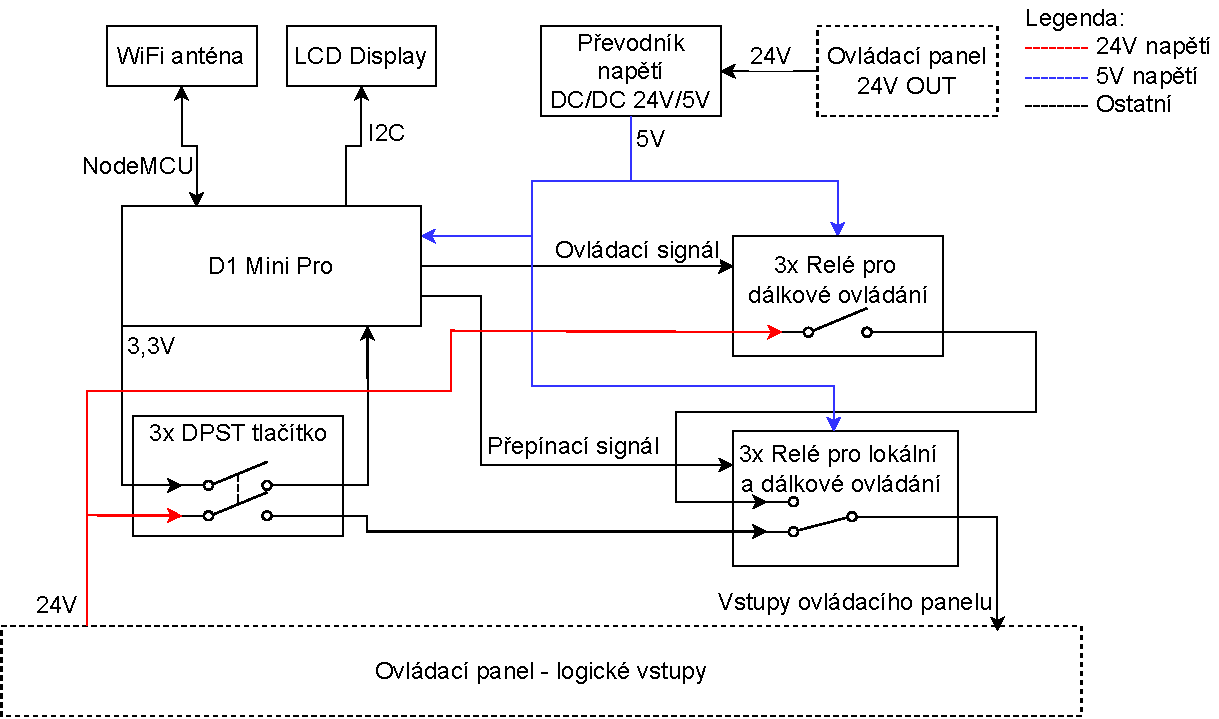
\includegraphics[width=0.99\linewidth]{Electrical_Schematic_V2.drawio.pdf}
			\caption{Schéma jednotlivých bloků v DPS}
			\label{fig:pcb_layout}
		\end{figure}
		
		\clearpage
			
		
		\item \textbf{Zpracujte pro něj kvalitativní analýzu FMECA (Failure Mode, Effects and Criticality Analysis). Analýza nemusí pokrývat všechny části objektu, minimální počet možných způsobů poruchy (failure modes) je 10, typický rozsah 1 strana A4. Určujte i Failure Risk Priority Number.}
		
		Z analýzy lze vidět, že nejhorší potenciální porucha jsou studené spoje během pájení. Proto by bylo rozumné upravit návrh desky (pokud na to je čas a peníze) a použít čipy, které podporují boundary scan a JTAG. Pomocí toho se dá zautomatizovat kontrola zapájení součástek pomocí interconnection testu.
		
		Z analýzy poté vyplývají ještě další možnost vylepšení návrhu systému jako je úprava designu krabičky nebo přidání senzorů na volné GPIO piny. Mimo to obsahuje i nějaké body ke kontrole při montáži.
		
		\clearpage
				
		\item \textbf{Pro jeden způsob selhání zvoleného objektu vytvořte strom poruch (Fault Tree Analysis).}
		
		Zvolil jsem si typ selhání "Neovladatelný systém" - kritický stav systému kdy není možné ovládat systém podle potřeby.
		
		Systém je navržený ve smyslu bezpečného selhání, což je důležitá informace nezahrnuta v FTA diagramu. Pokud ovládací panel přestane dostávat signály, bude nejdéle 30 sekund zpomalovat až do zastavení. Alternativně systém obsahuje i E-STOP který přímo zastavuje motory napojené na frekvenční měnič.
		
		Z grafu lze vidět, že už v systému jsou navrhnuty bezpečnostní prvky aby se systém nestal neovladatelným. Bylo by potřeba velké množství nepravděpodobných selhání aby došlo k nebezpečné situaci. 
		
		V návrhu není žádná redundance, protože kritický parametr systému byla cena.
		
		Systém taky obsahuje hodně podsystémů (značené trojúhelníky), které mají vlastní možné módy selhání.
		
	\end{enumerate}
	
	\printbibliography
	
\end{document}